\section{Introduction}
\label{sec:intro}

Recommender systems have emerged as fundamental infrastructure powering personalized experiences across digital platforms, influencing billions of user decisions daily. From e-commerce platforms processing millions of transactions to streaming services delivering content to global audiences, these systems have evolved far beyond simple collaborative filtering algorithms into sophisticated machine learning pipelines that adapt to user behavior in real-time~\cite{ricci2015recommender,adomavicius2005toward}.

The effectiveness of any recommender system fundamentally depends on its ability to accurately infer user preferences from available signals. This inference process relies critically on user feedback—the observable traces of user-item interactions that reveal underlying preferences and drive algorithmic learning. The nature, quality, and characteristics of this feedback data directly determine system performance, user satisfaction, and business outcomes~\cite{hu2008collaborative,herlocker2004evaluating}.

\begin{figure}[ht]
\centering
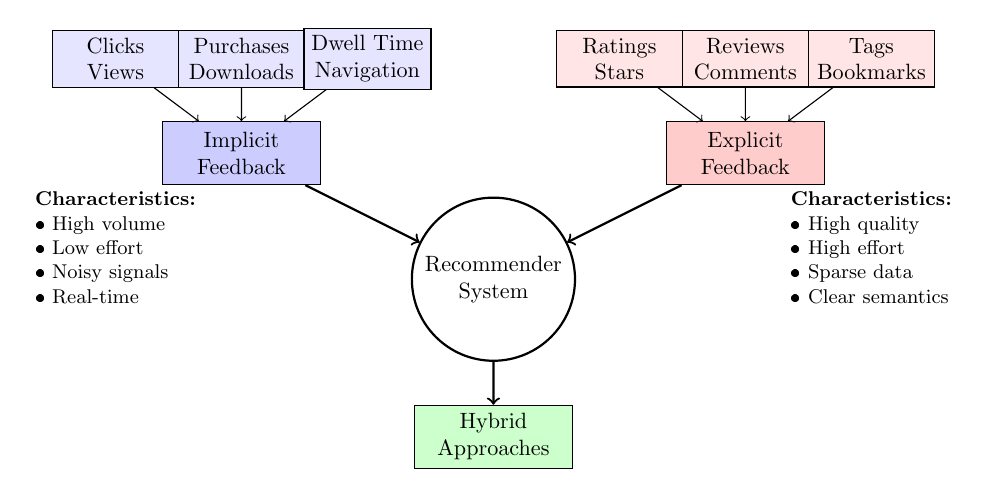
\begin{tikzpicture}[scale=0.8, transform shape]
    % Central circle
    \node[circle, draw, thick, minimum size=2cm, align=center] (center) at (0,0) {Recommender\\System};
    
    % Implicit feedback branch
    \node[rectangle, draw, fill=blue!20, minimum width=2.5cm, minimum height=1cm, align=center] (implicit) at (-4,2) {Implicit\\Feedback};
    \node[rectangle, draw, fill=blue!10, minimum width=2cm, minimum height=0.7cm, align=center] (clicks) at (-6,3.5) {Clicks\\Views};
    \node[rectangle, draw, fill=blue!10, minimum width=2cm, minimum height=0.7cm, align=center] (purchase) at (-4,3.5) {Purchases\\Downloads};
    \node[rectangle, draw, fill=blue!10, minimum width=2cm, minimum height=0.7cm, align=center] (time) at (-2,3.5) {Dwell Time\\Navigation};
    
    % Explicit feedback branch
    \node[rectangle, draw, fill=red!20, minimum width=2.5cm, minimum height=1cm, align=center] (explicit) at (4,2) {Explicit\\Feedback};
    \node[rectangle, draw, fill=red!10, minimum width=2cm, minimum height=0.7cm, align=center] (ratings) at (2,3.5) {Ratings\\Stars};
    \node[rectangle, draw, fill=red!10, minimum width=2cm, minimum height=0.7cm, align=center] (reviews) at (4,3.5) {Reviews\\Comments};
    \node[rectangle, draw, fill=red!10, minimum width=2cm, minimum height=0.7cm, align=center] (tags) at (6,3.5) {Tags\\Bookmarks};
    
    % Hybrid approach
    \node[rectangle, draw, fill=green!20, minimum width=2.5cm, minimum height=1cm, align=center] (hybrid) at (0,-2.5) {Hybrid\\Approaches};
    
    % Arrows
    \draw[thick, ->] (implicit) -- (center);
    \draw[thick, ->] (explicit) -- (center);
    \draw[thick, ->] (center) -- (hybrid);
    
    % Sub-connections
    \draw[->] (clicks) -- (implicit);
    \draw[->] (purchase) -- (implicit);
    \draw[->] (time) -- (implicit);
    \draw[->] (ratings) -- (explicit);
    \draw[->] (reviews) -- (explicit);
    \draw[->] (tags) -- (explicit);
    
    % Characteristics labels
    \node[align=left, font=\small] at (-6,0.5) {\textbf{Characteristics:}\\• High volume\\• Low effort\\• Noisy signals\\• Real-time};
    \node[align=left, font=\small] at (6,0.5) {\textbf{Characteristics:}\\• High quality\\• High effort\\• Sparse data\\• Clear semantics};
    
\end{tikzpicture}
\caption{Conceptual Framework: Feedback Types in Recommender Systems}
\label{fig:feedback_framework}
\end{figure}

\subsection{The Feedback Dichotomy: A Fundamental Design Choice}

User feedback in recommender systems is traditionally categorized into two fundamental types that represent distinct paradigms for preference elicitation and modeling, as illustrated in Figure~\ref{fig:feedback_framework}:

\textbf{Implicit feedback} encompasses user behaviors automatically captured through digital interactions without requiring conscious effort from users. These signals—including clicks, views, purchases, and dwell times—are abundant and enable real-time adaptation but suffer from inherent noise and ambiguity in preference interpretation~\cite{hu2008collaborative,pan2008one}.

\textbf{Explicit feedback} involves deliberate user actions to express preferences, such as ratings, reviews, and direct comparisons. While providing clear semantic meaning about user tastes, explicit feedback is typically sparse due to the cognitive effort required, leading to coverage limitations and potential selection biases~\cite{herlocker2004evaluating,adomavicius2005toward}.

This dichotomy represents more than a simple data classification—it reflects fundamental trade-offs in system design, user experience, computational requirements, and business models. The choice between feedback types affects algorithmic approaches, evaluation methodologies, privacy considerations, and ultimately, the success of deployed systems.

\subsection{Research Motivation: Critical Gaps and Challenges}

Despite three decades of research in recommender systems, several critical gaps persist in our understanding of feedback mechanisms and their optimal utilization:

\subsubsection{Lack of Unified Theoretical Framework}
Current literature treats implicit and explicit feedback as separate research streams, with limited systematic comparison of their fundamental properties, trade-offs, and optimal application contexts. This fragmentation hinders principled system design and fair algorithmic comparison.

\subsubsection{Inadequate Evaluation Methodologies}
Standard evaluation approaches often fail to account for feedback-specific characteristics, leading to biased comparisons between systems using different feedback types. Metrics designed for explicit feedback may not adequately capture the effectiveness of implicit feedback systems, and vice versa.

\subsubsection{Limited Understanding of Hybrid Integration}
While hybrid systems combining multiple feedback types show promise, principled approaches for integration remain underdeveloped. Critical questions persist about optimal combination strategies, conflict resolution, and the relative weighting of different signal types.

\subsubsection{Emerging Privacy and Fairness Concerns}
Modern privacy regulations and fairness considerations create new constraints on feedback collection and utilization. The differential privacy implications of implicit versus explicit feedback, along with their impact on algorithmic bias, require systematic investigation.

\subsection{Research Objectives and Contributions}

This survey addresses these gaps through a comprehensive analysis that establishes a unified framework for understanding implicit and explicit feedback in recommender systems. Our primary research objectives are:

\begin{enumerate}
    \item \textbf{Develop Unified Taxonomy}: Create a comprehensive framework for characterizing feedback types across multiple dimensions
    \item \textbf{Systematic Algorithmic Analysis}: Categorize and compare algorithmic approaches for different feedback types
    \item \textbf{Evaluation Framework}: Establish methodologies for fair comparison across feedback types
    \item \textbf{Domain Analysis}: Examine feedback characteristics and optimal strategies across application domains
    \item \textbf{Research Roadmap}: Identify critical challenges and future research directions
\end{enumerate}

\subsection{Survey Contributions}

This survey makes several key contributions to the recommender systems field:

\subsubsection{Unified Taxonomy and Analysis Framework}
We present a comprehensive taxonomy that characterizes feedback along five key dimensions: collection mechanism, signal quality, temporal characteristics, user cognitive load, and privacy implications. This framework enables systematic comparison of feedback types and guides system design decisions.

\subsubsection{Comprehensive Algorithmic Review}
Through systematic analysis of 147 research papers, we identify and categorize fundamental algorithmic paradigms for each feedback type, revealing key insights about their relative effectiveness, computational requirements, and applicability across domains.

\subsubsection{Evaluation Framework Analysis}
We examine evaluation methodologies that account for feedback-specific characteristics, enabling fair comparison between systems using different feedback types. Our analysis addresses selection bias, temporal dynamics, and domain-specific considerations.

\subsubsection{Empirical Domain Analysis}
We provide systematic analysis of how feedback characteristics influence system design across major application domains, revealing domain-specific patterns and deployment strategies.

\subsubsection{Research Roadmap}
We identify critical research directions for feedback-aware recommender systems: bias-aware evaluation, privacy-preserving collection, real-time hybrid integration, and fair representation.

\subsection{Scope and Methodology}

This survey synthesizes research spanning 2010-2025, focusing on the period when implicit feedback gained prominence and hybrid approaches emerged. Our methodology includes:

\begin{itemize}
    \item \textbf{Systematic Literature Review}: Analysis of 147 papers from top-tier venues including ACM RecSys, WWW, SIGIR, KDD, and domain-specific journals
    \item \textbf{Algorithmic Classification}: Comprehensive taxonomy organizing approaches by feedback type, methodology, and application domain
    \item \textbf{Empirical Analysis}: Examination of real-world system deployments across e-commerce, streaming, social media, and other domains
    \item \textbf{Comparative Evaluation}: Systematic comparison of approaches using standardized metrics and datasets where available
\end{itemize}

\subsection{Paper Organization}

This survey is structured to provide comprehensive coverage of feedback mechanisms:

\begin{itemize}
    \item \textbf{Section~\ref{sec:survey_methodology}} outlines our systematic survey methodology and literature review approach
    \item \textbf{Section~\ref{sec:related}} provides comprehensive background and positions our work within the broader literature
    \item \textbf{Section~\ref{sec:methodology}} presents our unified taxonomy and systematic analysis of algorithmic approaches
    \item \textbf{Section~\ref{sec:evaluation}} examines evaluation frameworks and bias analysis methodologies
    \item \textbf{Section~\ref{sec:applications}} explores real-world deployments across diverse application domains
    \item \textbf{Section~\ref{sec:challenges}} identifies critical challenges and future research directions
    \item \textbf{Section~\ref{sec:conclusion}} synthesizes key insights and provides actionable recommendations
\end{itemize}

\subsection{Target Audience and Impact}

This survey targets multiple stakeholders in the recommender systems ecosystem:

\begin{itemize}
    \item \textbf{Researchers} seeking comprehensive understanding of feedback mechanisms and identification of research opportunities
    \item \textbf{System Architects} designing production recommender systems and making informed technology choices
    \item \textbf{Data Scientists} developing and deploying recommendation algorithms in real-world applications
    \item \textbf{Students and Practitioners} learning about personalization technologies and their practical implementation
\end{itemize}

By establishing a unified theoretical foundation and providing practical guidance, this work aims to advance both the scientific understanding and practical deployment of feedback-aware recommender systems.